\documentclass[10pt,letterpaper,twocolumn]{article}
\usepackage[margin=0.78in,columnsep=0.24in]{geometry}
\usepackage[T1]{fontenc}
\usepackage{lmodern}
\usepackage{microtype}
\usepackage{graphicx}
\usepackage{booktabs}
\usepackage{amsmath}
\usepackage{caption}
\usepackage{float}
\usepackage[hidelinks]{hyperref}
\usepackage{enumitem}
\setlength{\parindent}{1em}
\setlength{\parskip}{0pt}
\setlength{\textfloatsep}{9pt plus 2pt minus 2pt}
\setlength{\intextsep}{8pt plus 2pt minus 2pt}
\raggedbottom
\captionsetup{font=small,labelfont=bf,justification=raggedright,singlelinecheck=false}
\renewcommand{\refname}{References}
\renewcommand{\thesection}{\arabic{section}}
\title{\vspace{-1.15cm}\bfseries\large Computational Investigation of Radiation-Induced Vacancy Formation and Multi-Objective Screening of Inorganic Halide Perovskites}
\author{Abiha Saqib}
\date{}
\begin{document}
\twocolumn[{
\begin{@twocolumnfalse}
\maketitle
\vspace{-1.4em}
\noindent\textbf{Abstract}\par\smallskip
\noindent\small
Understanding radiation-associated point defects and selecting candidate materials are complementary challenges in the study of inorganic halide perovskites. Existing depth-dependent simulation profiles for CsPbI$_3$ and Cs$_3$Sb$_2$I$_9$ were analyzed at 20, 50, 100, and 500 keV. A multilayer perceptron (MLP) was evaluated for prediction of Cs-, B-site-, and I-vacancy profiles using held-out irradiation energies and simple baselines. The observed vacancy maxima generally shifted toward greater depths between 20 and 100 keV. Averaged across six material--species outcomes, an improved MLP achieved a lower root mean squared error (RMSE) than a zero-prediction baseline at 20, 50, and 100 keV, but not at 500 keV. Materials Project queries for seven candidate compositions returned 15 phase records, and phase-specific Pareto analysis identified Cs$_2$AgInCl$_6$ (mp-1096926) and Cs$_3$Sb$_2$I$_9$ (mp-541014) as non-dominated under the reference screening objectives. A 30-scenario sensitivity analysis provided conditional prioritization. These results outline a limited-data computational workflow linking vacancy-profile prediction with electronic--thermodynamic materials screening, without claiming radiation resistance for compounds lacking irradiation data.

\vspace{0.65em}\noindent\textbf{Keywords:} inorganic halide perovskites; vacancies; irradiation; machine learning; Materials Project; Pareto screening.
\vspace{1.2em}
\end{@twocolumnfalse}
}]

\section{Introduction}
Inorganic halide perovskites and related compounds are of interest for photovoltaic and optoelectronic applications because their composition and structure influence electronic properties. Interest in space and other radiation-exposed environments has motivated direct proton-irradiation studies. Experiments on perovskite tandem photovoltaics and targeted proton exposure demonstrate that the response depends on irradiation energy, fluence, device architecture, and defect-related mechanisms \cite{lang2020,durant2021}. Radiation-induced ion migration and void formation have also been reported \cite{nguyen2024}. These device-level findings do not necessarily transfer to other compositions.

Depth-resolved radiation calculations provide information on spatial variation in vacancy-related events. Their interpretation depends on the projectile, displacement thresholds, target density, fluence, and normalization convention. Extending simulations across many materials and energies can be costly. Predictive modelling may help characterize patterns in available outputs, but random division of closely related depth points risks overstating generalization. Whole-energy holdout evaluation is therefore essential.

Computed electronic descriptors offer a complementary pathway for material selection. The Materials Project provides phase-specific electronic and thermodynamic information \cite{horton2025}. These calculations can support candidate screening, although computed electronic gaps and energies above hull are not direct measurements of optical absorption, synthesis feasibility, or radiation endurance. The photovoltaic response of Cs$_3$Sb$_2$I$_9$, for example, is strongly dependent on structural dimensionality \cite{guo2025}.

Here we combine (i) energy-dependent vacancy-profile analysis and neural-network evaluation for CsPbI$_3$ and Cs$_3$Sb$_2$I$_9$ with (ii) multi-objective screening of additional inorganic halide perovskite phases. The aim is to characterize what can be inferred from existing datasets and define a defensible candidate shortlist.

\section{Materials and Methods}
\subsection{Radiation simulation dataset}
The source workbook contained eight material--energy profiles: CsPbI$_3$ and Cs$_3$Sb$_2$I$_9$, each at 20, 50, 100, and 500 keV. Cleaning yielded 796 depth records. Seven profiles contained 100 depth samples; the CsPbI$_3$ 100 keV profile contained 96. Each row contained depth in \AA, energy, material identity, and three vacancy channels for Cs, the B-site element (Pb or Sb), and I. Reported vacancy amplitudes are retained in their source normalization because the original irradiation fluence and physical vacancy-unit definition remain unverified.

Peak profile value, peak depth, and mean value were calculated for each material--energy--species combination. Numerical profile areas were obtained through trapezoidal integration over the recorded depth interval. These integrals, expressed in reported units times \AA, are descriptive and should not be interpreted as absolute vacancy yields.

\subsection{Predictive model and validation}
Predictors were energy, depth, and two material-indicator variables. The original MLP comprised hidden dense layers of 64, 64, and 32 ReLU neurons with three linear outputs. The improved configuration used $\log_{10}(E)$ and a Softplus output to enforce nonnegative predictions. Inputs were standardized on training data alone; improved target channels were scaled by the respective training-set 95th-percentile values. Both models used Adam at a learning rate of 0.001, mean squared error loss, and batch size 32.

For each evaluation, one irradiation energy was withheld for both materials. One of the three remaining energies was used for selection of the training duration (up to 500 epochs, early-stopping patience 35); the final network was refitted using all three available energies. The notebook used seeds 42--46. Evaluation used MAE, RMSE, and $R^2$, supplemented by zero prediction, nearest-energy, linear-energy, and log-energy baselines. Depth interpolation was scored only over coordinates supported by reference profiles.

\subsection{Multi-objective material screening}
Materials Project queries for seven compositions returned 15 phase records. Initial eligibility required a computed band gap between 1.0 and 2.2 eV and energy above hull at most 0.05 eV atom$^{-1}$. Five records met these two conditions. Direct/indirect gap character was recorded but not used as an exclusion criterion. The reference Pareto objectives minimized the absolute difference from a 1.5 eV target gap and minimized energy above hull.

Sensitivity was evaluated over 30 combinations: gap targets 1.3, 1.5, and 1.7 eV; hull thresholds 0, 0.003, 0.005, 0.01, and 0.025 eV atom$^{-1}$; and gap ranges 1.0--2.2 or 1.2--1.8 eV. Selection frequency was calculated relative to the number of scenarios where the phase was eligible. Some scenarios contained only one eligible candidate and are not evidence of pairwise superiority.

\section{Results}
\subsection{Vacancy distributions}
The primary maxima shifted deeper in both materials between 20 and 100 keV (Fig.~\ref{fig:profiles}). At 500 keV, small-amplitude, distributed features complicate interpretation and several estimated maxima lie near the 10,000 \AA\ depth boundary. The Cs-vacancy peak of CsPbI$_3$ at 100 keV is unusually strong compared with the other tested energies and warrants confirmation against the original simulation settings.

\begin{figure}[H]
\centering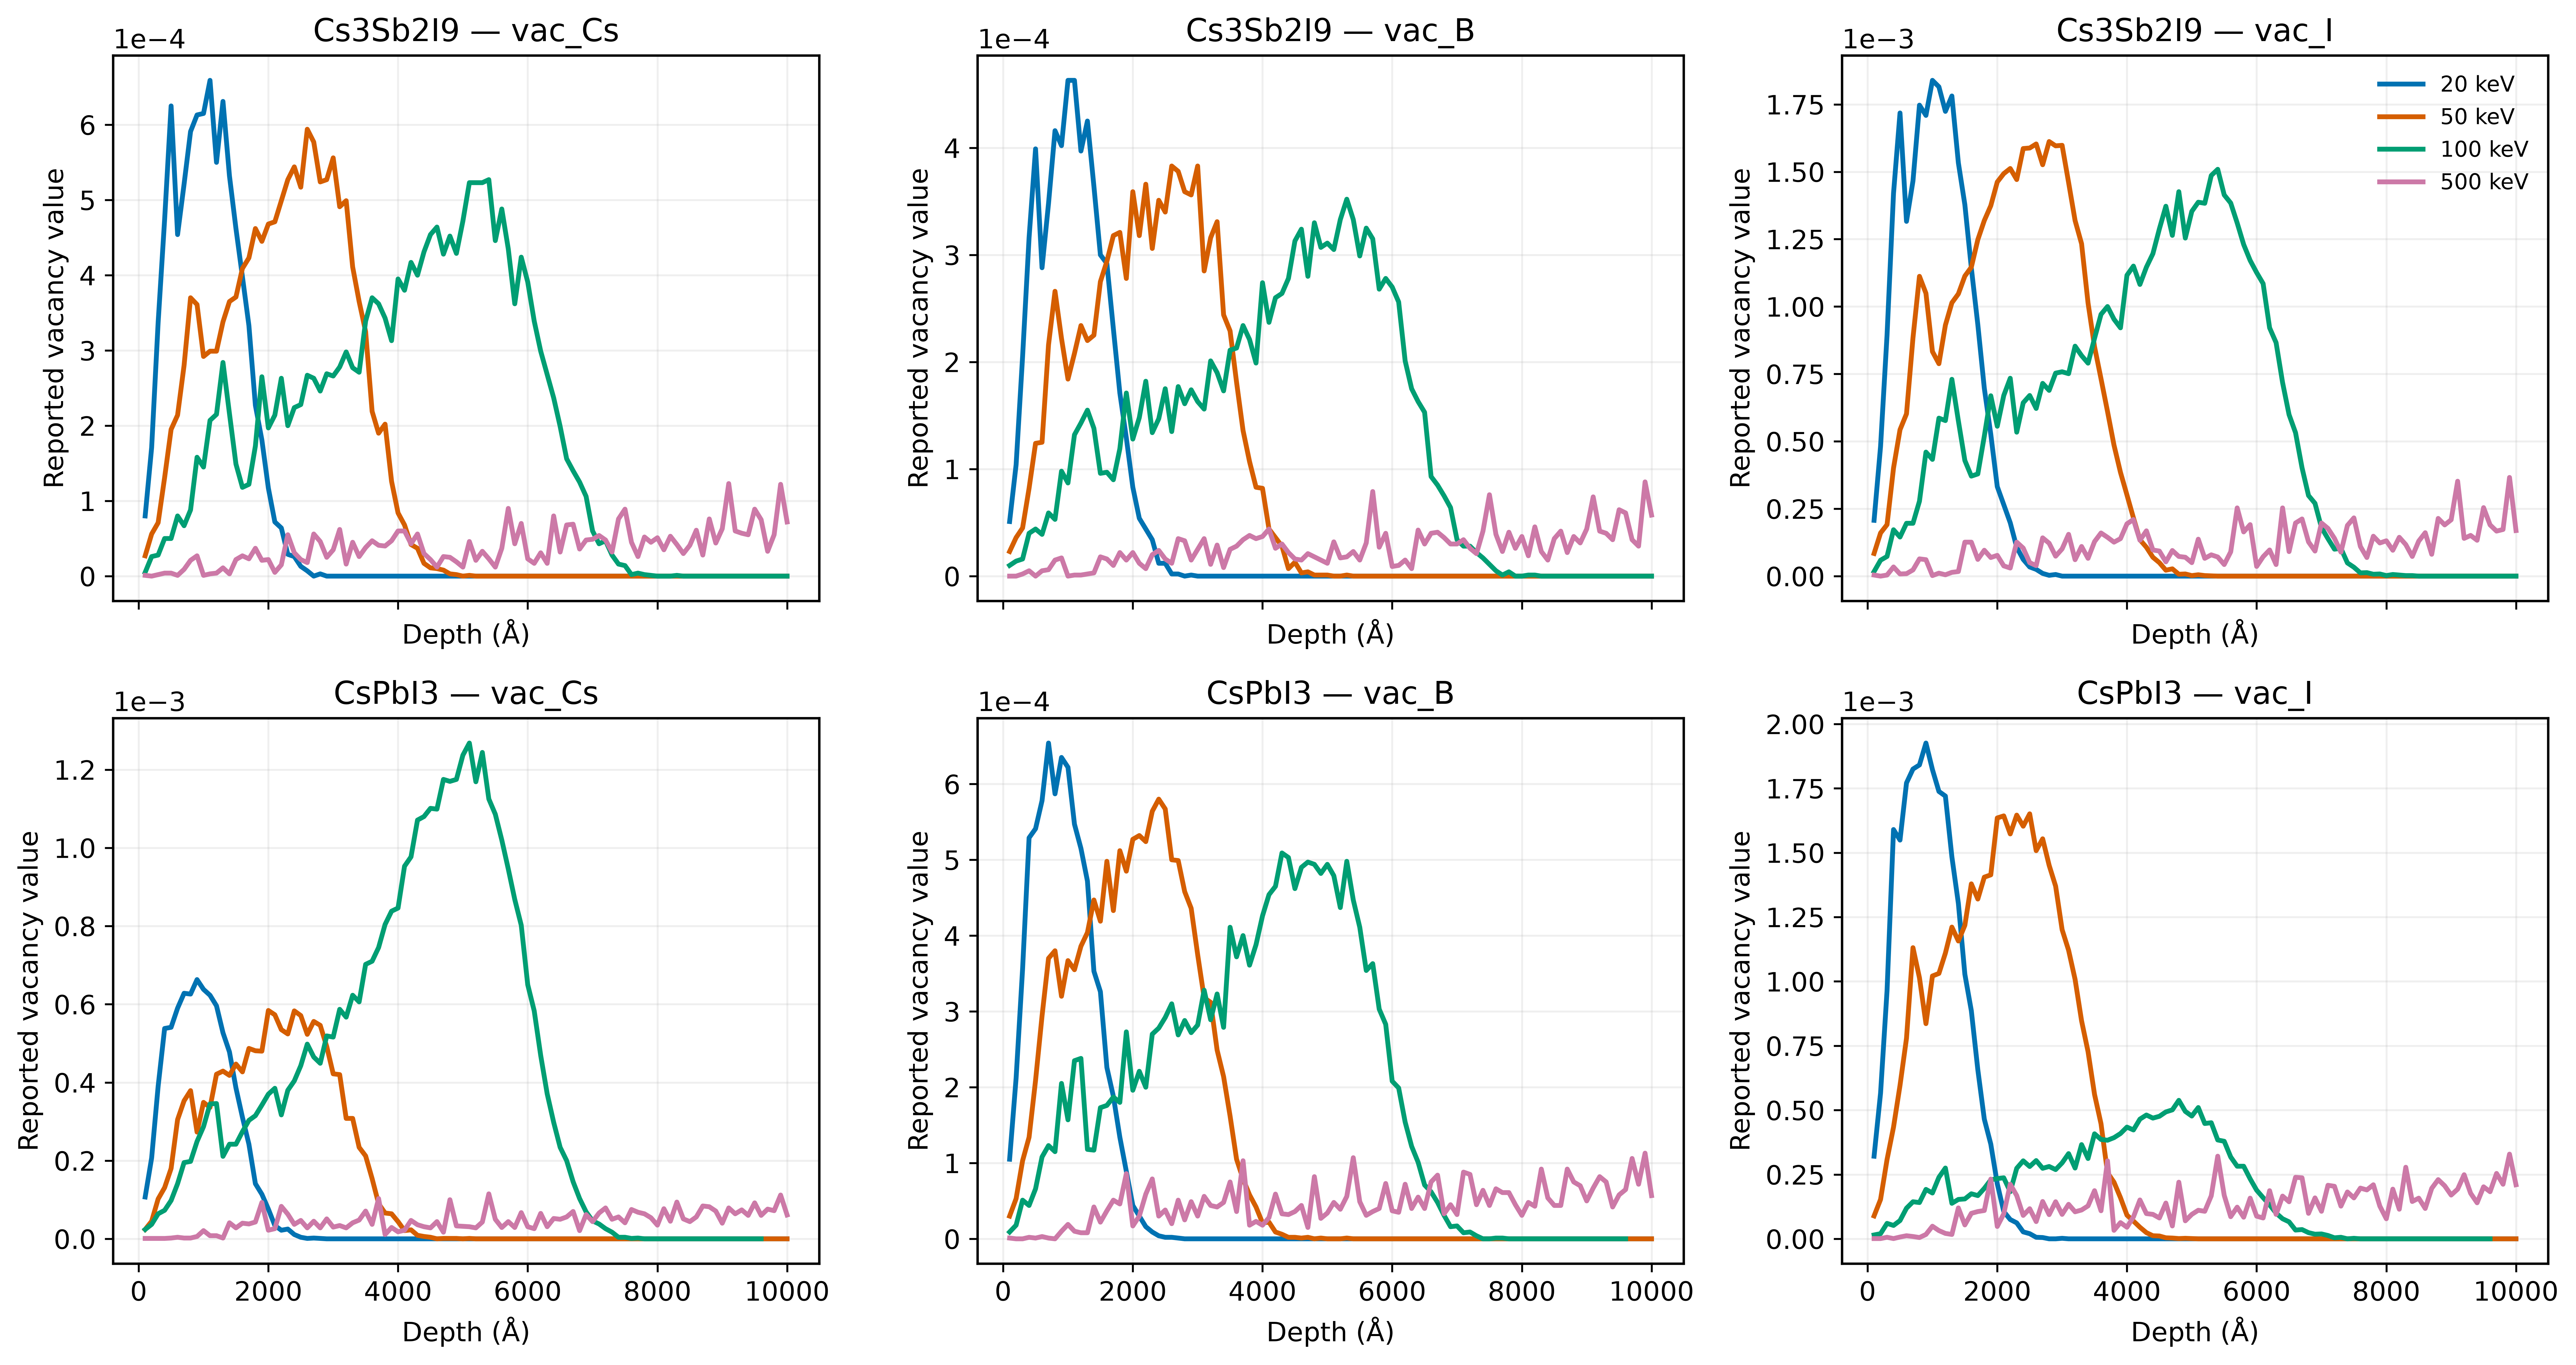
\includegraphics[width=\columnwidth]{figures/Figure_1_Vacancy_Profiles.png}
\caption{Reported Cs-, B-site-, and I-vacancy profiles for CsPbI$_3$ and Cs$_3$Sb$_2$I$_9$ at four irradiation energies. Values retain the simulation's unverified normalization.}\label{fig:profiles}
\end{figure}

\subsection{Depth localization and profile integrals}
The iodine-vacancy maximum moved from 1,000 to 5,400 \AA\ in Cs$_3$Sb$_2$I$_9$ and from 900 to 4,800 \AA\ in CsPbI$_3$ between 20 and 100 keV (Fig.~\ref{fig:depth}). Cs-vacancy maxima shifted from 1,100 to 5,400 \AA\ and from 900 to 5,100 \AA, respectively. Several 500 keV maxima occurred at approximately 9,900 \AA, near the last recorded point.

\begin{figure}[H]
\centering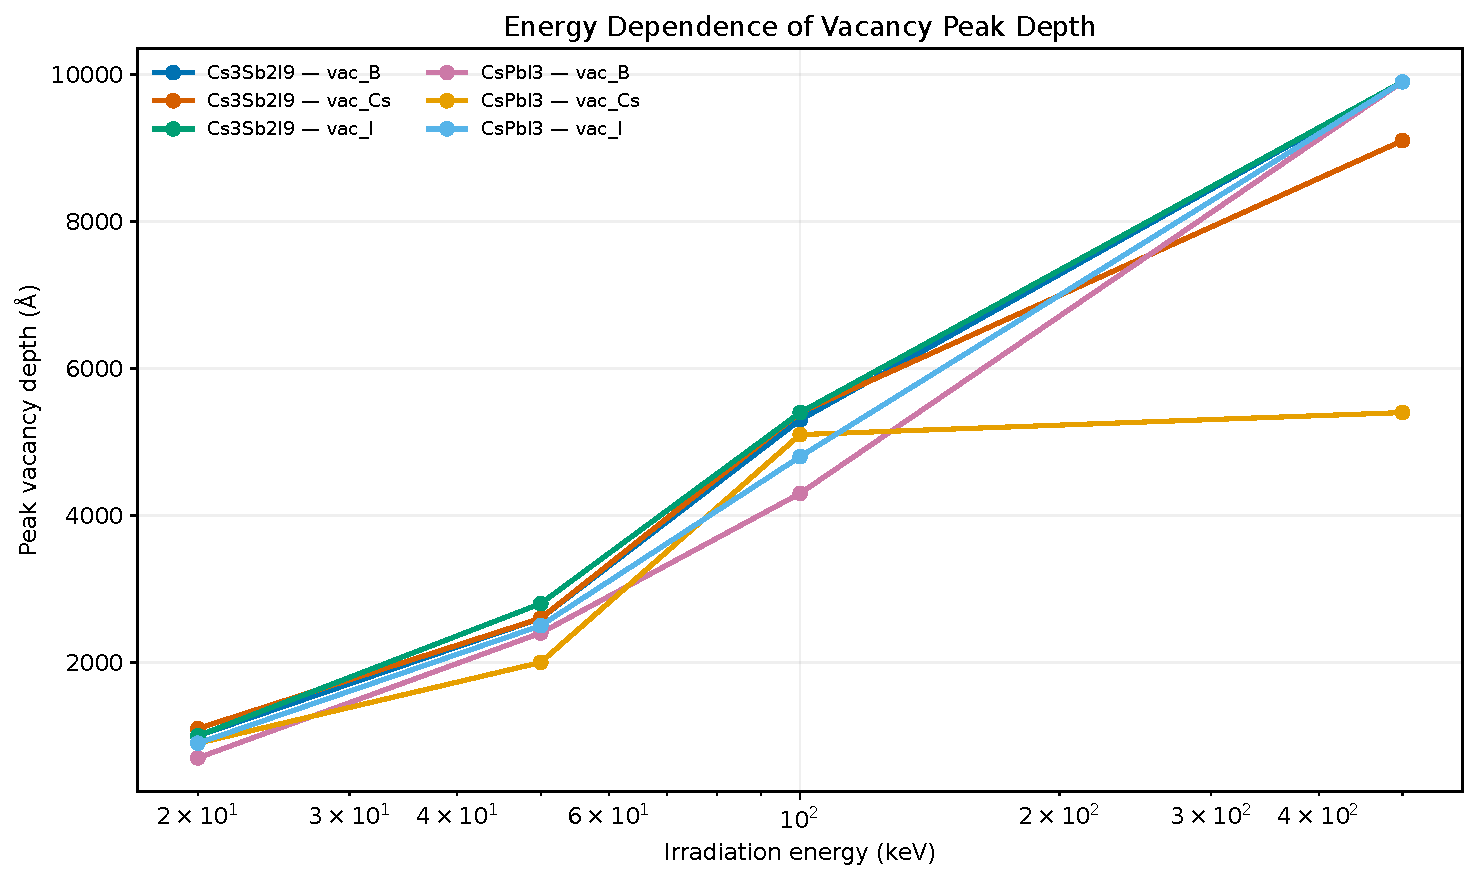
\includegraphics[width=\columnwidth]{figures/Figure_2_Peak_Depth.pdf}
\caption{Peak vacancy depth versus incident energy. Points close to the maximum sampled depth are potentially affected by window truncation.}\label{fig:depth}
\end{figure}

For the Cs$_3$Sb$_2$I$_9$ iodine channel, the integrated recorded profile increased from 2.53 at 20 keV to 5.55 reported units\,$\times$\,\AA\ at 100 keV, and decreased to 1.13 at 500 keV (Fig.~\ref{fig:int}). This is a recorded-window integral, not a claim of reduced total defects at higher irradiation energies.

\begin{figure}[H]
\centering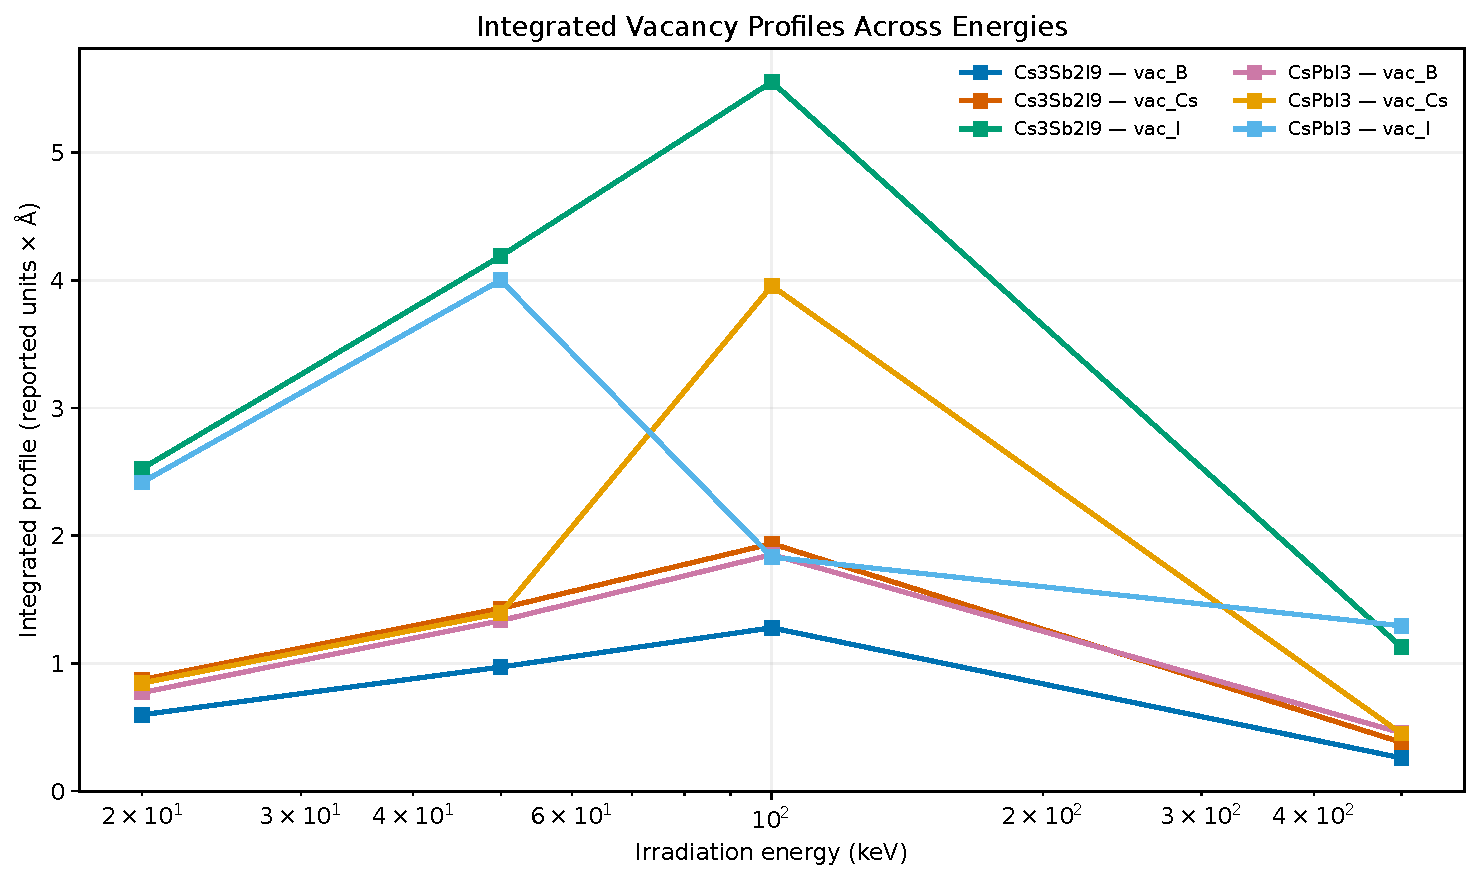
\includegraphics[width=\columnwidth]{figures/Figure_3_Integrated_Profiles.pdf}
\caption{Trapezoidal integrals of reported depth profiles. Physical defect-yield interpretation requires the original normalization and full depth extent.}\label{fig:int}
\end{figure}

\subsection{Held-out predictive performance}
The improved MLP had lower average RMSE than the zero baseline at 20, 50, and 100 keV, but the zero baseline was considerably stronger at 500 keV (Table~\ref{tab:rmse}; Fig.~\ref{fig:rmse}). Aggregates span six material--species outcomes and can conceal heterogeneous performance within individual channels.

\begin{table}[H]
\caption{Average held-out RMSE over six material--species combinations.}\label{tab:rmse}
\centering\small
\begin{tabular}{rrrr}
\toprule
Energy (keV)&Improved MLP&Zero baseline&Better\\
\midrule
20&0.000290&0.000329&MLP\\
50&0.000315&0.000390&MLP\\
100&0.000316&0.000378&MLP\\
500&0.000334&0.000076&Zero\\
\bottomrule
\end{tabular}
\end{table}

\begin{figure}[H]
\centering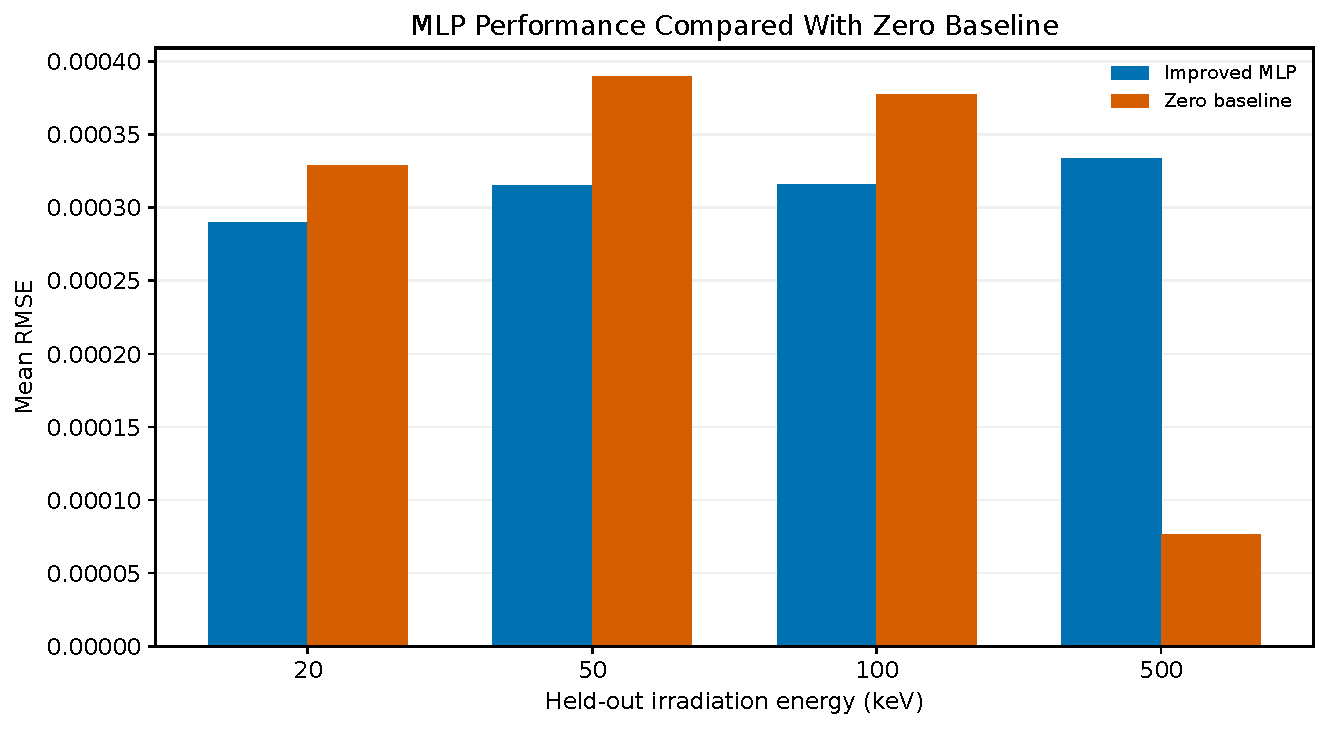
\includegraphics[width=\columnwidth]{figures/Figure_4_Model_Performance.pdf}
\caption{Mean RMSE of the improved MLP and zero baseline under held-out irradiation energies.}\label{fig:rmse}
\end{figure}

\subsection{Electronic and thermodynamic screening}
The two non-dominated records under the reference objectives were Cs$_3$Sb$_2$I$_9$ (mp-541014, gap 1.5406 eV, hull 0.003167 eV atom$^{-1}$) and Cs$_2$AgInCl$_6$ (mp-1096926, computed gap 1.3422 eV, hull 0). All five initially eligible phases had an indirect calculated gap in the returned data. Electronic-structure predictions should not be equated to experimental optical gaps, particularly for Cs$_2$AgInCl$_6$ and doped variants \cite{li2024}.

\begin{table}[H]
\caption{Pareto appearances among eligible parameter scenarios.}\label{tab:pareto}
\centering\small
\begin{tabular}{lrr}
\toprule
Phase ID&Count&Rate\\
\midrule
Cs$_2$AgInCl$_6$ (mp-1096926)&25/30&83.3\%\\
Cs$_3$Sb$_2$I$_9$ (mp-541014)&12/18&66.7\%\\
Cs$_3$Sb$_2$I$_9$ (mp-23029)&5/15&33.3\%\\
Cs$_2$AgBiBr$_6$ (mp-1078250)&0/12&0\%\\
CsSnI$_3$ (mp-27381)&0/9&0\%\\
\bottomrule
\end{tabular}
\end{table}

\begin{figure}[H]
\centering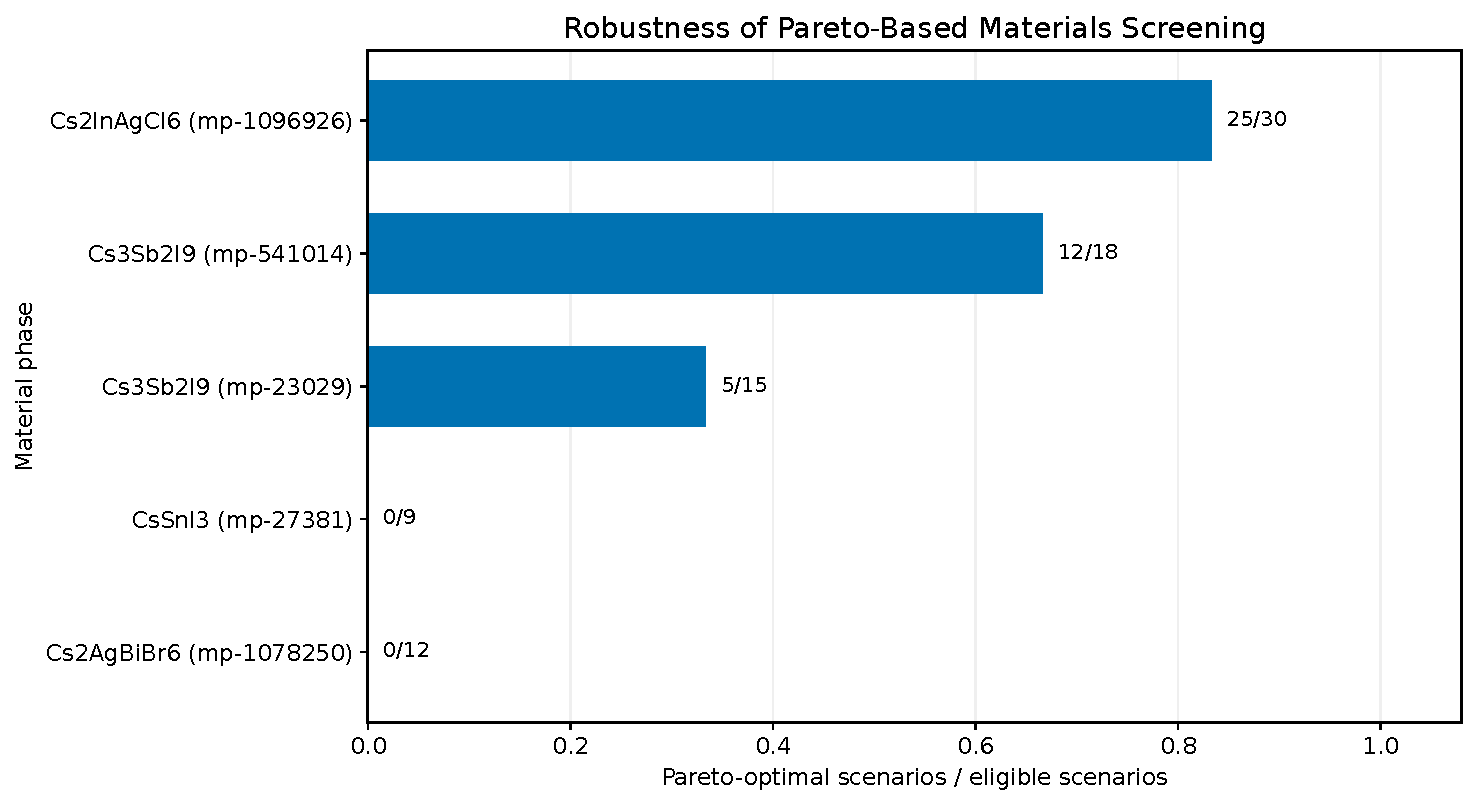
\includegraphics[width=\columnwidth]{figures/Figure_5_Pareto_Robustness.pdf}
\caption{Conditional Pareto selection frequencies for distinct phase records. Fractions refer to eligible scenarios, not comparative radiation tolerance.}\label{fig:pareto}
\end{figure}

\section{Discussion}
\subsection{Interpretation of irradiation profiles}
The most consistent physical observation is the deeper location of prominent vacancy features from 20 to 100 keV. The precise mechanism cannot be established without the simulation conditions. The finite sampled range complicates 500 keV interpretations, while the 100 keV CsPbI$_3$ Cs-vacancy amplitude requires source verification.

\subsection{Limits of predictive generalization}
The 796 depth rows represent only eight independent material--energy profiles. Whole-energy holdouts therefore avoid a potentially misleading random-row evaluation. Although the MLP was useful under certain held-out energies, its 500 keV behavior argues against broad extrapolation claims. This negative result is scientifically informative and highlights the value of strong baseline comparisons.

\subsection{Screening and published evidence}
The screened objectives concern calculated electronic and thermodynamic properties, not radiation resistance. Cs$_3$Sb$_2$I$_9$ connects the irradiation profiles with reported phase-dependent photovoltaic research \cite{guo2025}. Cs$_2$AgInCl$_6$ is a conditional computational shortlist candidate; optical properties in the literature remain structure- and synthesis-dependent \cite{li2024}. Al-doping device-oriented simulations for Cs$_2$AgBiBr$_6$ \cite{ullah2024} and experimental CsSnI$_3$ photovoltaic work \cite{ye2021} provide application context, but no basis for a radiation-hardness ranking of the screened phases.

\subsection{Limitations}
Important limitations include unverified vacancy units, incident projectile and fluence information, only two irradiated compositions and four energies, possible high-energy profile truncation, phase-specific differences between database and experimental materials, and the limited set of screening objectives. No new radiation simulations were conducted for the additional screened candidates.

\section{Conclusions}
The existing irradiation profiles establish energy-dependent vacancy localization and provide a compact test bed for held-out-energy MLP prediction. The MLP improves average error relative to zero prediction at three energies but fails at 500 keV. Electronic--thermodynamic screening of 15 phase records identifies conditional Pareto candidates without demonstrating radiation hardness. The integrated methodology supports transparent candidate prioritization while clearly delineating the evidence needed for further physical validation.

\section*{Data Availability and Declarations}
The datasets, computational notebooks, source code, analysis results, and supporting figures associated with this study are available in the public GitHub repository: \url{https://github.com/abihasaqib24-lab/perovskite-radiation-study}. Reuse of any third-party source datasets remains subject to their respective permissions.

\noindent\textbf{Generative AI declaration.} Generative AI tools assisted with code debugging, visualization refinement, and manuscript editing; the author retains responsibility for the scientific analyses, interpretations, and conclusions.

\begin{thebibliography}{9}\small
\bibitem{lang2020} F. Lang \emph{et al.}, ``Proton Radiation Hardness of Perovskite Tandem Photovoltaics,'' \emph{Joule} \textbf{4}, 1054--1069 (2020). \href{https://doi.org/10.1016/j.joule.2020.03.006}{doi:10.1016/j.joule.2020.03.006}.
\bibitem{durant2021} B. K. Durant, H. Afshari, S. Singh \emph{et al.}, ``Tolerance of Perovskite Solar Cells to Targeted Proton Irradiation and Electronic Ionization Induced Healing,'' \emph{ACS Energy Lett.} \textbf{6}, 2362--2368 (2021). \href{https://doi.org/10.1021/acsenergylett.1c00756}{doi:10.1021/acsenergylett.1c00756}.
\bibitem{nguyen2024} D.-T. Nguyen, A. D. Bui, K. Huang \emph{et al.}, ``Void Formation and Radiation-Induced Ion Migration in Perovskite Solar Cells under 10 MeV Proton Radiation,'' \emph{Sol. RRL} \textbf{8}, 2400113 (2024). \href{https://doi.org/10.1002/solr.202400113}{doi:10.1002/solr.202400113}.
\bibitem{horton2025} M. K. Horton, P. Huck, R. X. Yang \emph{et al.}, ``Accelerated Data-Driven Materials Science with the Materials Project,'' \emph{Nat. Mater.} \textbf{24}, 1522--1532 (2025). \href{https://doi.org/10.1038/s41563-025-02272-0}{doi:10.1038/s41563-025-02272-0}.
\bibitem{guo2025} Y. Guo, F. Zhao, C. Zhang \emph{et al.}, ``Suppressing the Electron--Phonon Coupling in 2D Perovskite Cs3Sb2I9 for Lead-Free Indoor Photovoltaics,'' \emph{Adv. Sci.} \textbf{12}, e09281 (2025). \href{https://doi.org/10.1002/advs.202509281}{doi:10.1002/advs.202509281}.
\bibitem{li2024} Y. Li, J. Li, S. Ye \emph{et al.}, ``Cu$^+$-doped lead-free double perovskite quantum dots for enhancing the photovoltaic performance of carbon-based Cs2AgInCl6 perovskite solar cells,'' \emph{Phys. Chem. Chem. Phys.} \textbf{26}, 6984--6990 (2024). \href{https://doi.org/10.1039/D3CP05297D}{doi:10.1039/D3CP05297D}.
\bibitem{ullah2024} A. Ullah, M. I. Khan, Ihtisham-ul-Haq \emph{et al.}, ``Bandgap Engineering and Enhancing Optoelectronic Performance of a Lead-Free Double Perovskite Cs2AgBiBr6 Solar Cell via Al Doping,'' \emph{ACS Omega} \textbf{9}, 18202--18211 (2024). \href{https://doi.org/10.1021/acsomega.3c10388}{doi:10.1021/acsomega.3c10388}.
\bibitem{ye2021} T. Ye, K. Wang, Y. Hou \emph{et al.}, ``Ambient-Air-Stable Lead-Free CsSnI3 Solar Cells with Greater than 7.5\% Efficiency,'' \emph{J. Am. Chem. Soc.} \textbf{143}, 4319--4328 (2021). \href{https://doi.org/10.1021/jacs.0c13069}{doi:10.1021/jacs.0c13069}.
\end{thebibliography}
\end{document}
